\chapter{Logging}
\label{sec:module.Logging}

Nach einem absolvierten Spiel analysierten wir jeweils die Spielsituationen, welche sich ergeben haben. Dazu geh�rte das Analysieren des geschriebenen Logs. Dabei bedienten wir uns den nachfolgenden Mechanismen.

\section{Logkategorien und Loglevel}
\label{sec:module.Logging.LogkategorienundLoglevel}

Jeder Logeintrag geh�rt einer Logkategorie an. Je Logkategorie kann der Loglevel defniert werden. Die Loglevel lauten TRACE, DEBUG, INFO und ERROR. Wenn also zum Beispiel bei der Logkategorie ATTACKHILLMISSION der Loglevel auf INFO gestellt ist, werden nur die Fehler auf Stufe INFO und ERROR in das Logfile geschieben. Zudem kann, falls erw�nscht, jede Logkategorie in ein eigenes Logfile geschrieben werden. Die meisten Module habe ihre eigene Logkategorie, so kann durch korrekte Logeinstellung erzwungen werden dass nur die Logs, welche f�r das Analysieren eines bestimmten Spielmoduls von Bedeutung sind, ins Logfile geschrieben werden. Dadurch m�ssen nicht riesige Mengen an Logs druchw�lzt werden um an die Informationen heran zu kommen.


\section{JavaScript Addon f�r HMTL-Gameviewer}
\label{sec:module.Logging.Addon}
Das Codepaket welches von den Challenge-Organisatoren mitgeliefert wird, bietet bereits eine hilfreiche 2D-Visualisierung des Spiels, mit welchem das Spielgeschehen mitverfolgt werden kann. Die Visualisierung wurde mit HMTL und Javascript implementiert. Leider ist es nicht m�glich zus�tzliche Informationen auf die Seite zu projizieren. Deshalb haben wir den Viewer bereits im Projekt 2 mit einer solchen Funktion erweitert. Mit der Codezeile Logger.liveInfo(...) kann eine Zusatzinformation geschrieben werden, welche auf dem Viewer sp�ter sichtbar ist. Es muss definiert werden mit welchem Zug und wo auf dem Spielfeld die Infomation angezeigt werden soll. Im Beispiel wird an der Position der Ameise (ant.getTile()) ausgegeben welchen Task die Ameise hat.
\begin{verbatim}
Logger.liveInfo(Ants.getAnts().getTurn(), ant.getTile(), 
                "Task: %s ant: %s", issuer, ant.getTile());
\end{verbatim}
Auf der Karte wird ein einfaches aber praktisches Popup mit den geschriebenen Informationen angezeigt. Dank solcher Zusatzinformationen muss nicht m�hsam im Log nachgeschaut werden, welcher Ameise wann und wo welcher Task zugeordnet ist.

\begin{figure}[bth]
\centering
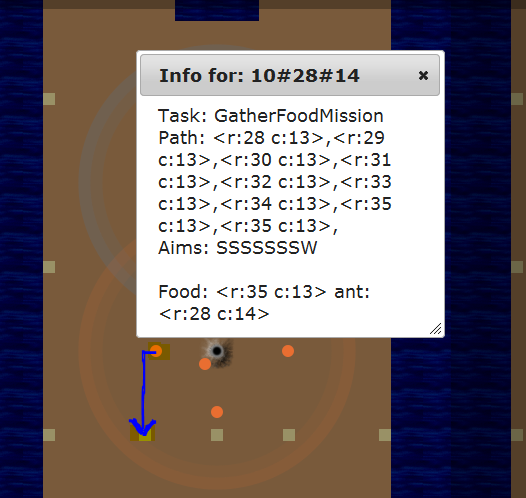
\includegraphics[height=70mm]{91_bilder/javascriptAddon.png}
\label{fig.javascriptAddon}
\caption[Live-Info Popupfenster]{Im Popupfenster steht die Aufgabe der Ameise sowie die Pixel des Pfades (falls vorhanden), welcher die Ameise ablaufen wird.}
\end{figure}

Das angezeigte Popup zeigt welchen Task (GatherFoodTask) die Ameise hat, wo sie sich befindet <r:28 c:14>, welches Futterpixel angesteuert wird <r:35 c:13> und welchen Pfad dazu berechnet wurde. Im Rahmen der Bachelorarbeit wurde dieses Addon erweitert. Nun werden alle Pixel welche in dem Popup ausgegeben werden auf der Karte markiert. Siehe (Abb. \ref{fig.javascriptAddon2})

\begin{figure}[bth]
\centering
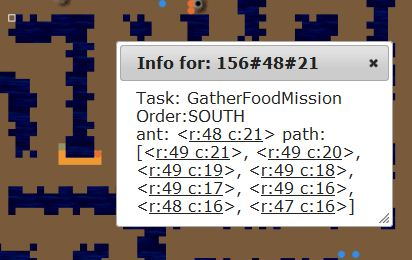
\includegraphics[height=45mm]{91_bilder/javascriptAddon2.jpg}
\label{fig.javascriptAddon2}
\caption[Erweiterung des Live-Info Popupfenster]{Mit der erweiterten Version wird der Pfad (orange) der Ameise von <r:48 c:21> nach <r:47 c:16> auf der Karte abgebildet.}
\end{figure}